\documentclass[t,aspectratio=169]{beamer}
%\usetheme{Berkeley}
\usepackage{graphicx}
\usepackage{amsmath}
\usepackage[american]{circuitikz}

\title{Clase 20}
\subtitle{Aplicaciones del transistor BJT}
\author{Dr.-Ing. Juan José Montero Rodríguez}
\subject{Elementos Activos}
\institute{Escuela de Ingeniería Electrónica}
\date{Semestre II-2023}

\begin{document}

\begin{frame}{}
\maketitle
\end{frame}

\section{Aplicaciones}
\begin{frame}{Controlador de relay}

\begin{figure}[H]
    \centering
    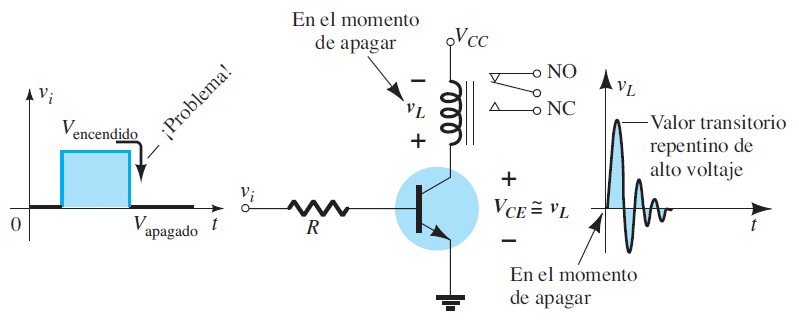
\includegraphics[width=\textwidth]{figuras/aplicaciones_1.png}
\end{figure}

\end{frame}


\begin{frame}{Controlador de relay con diodo de protección}

\begin{figure}[H]
    \centering
    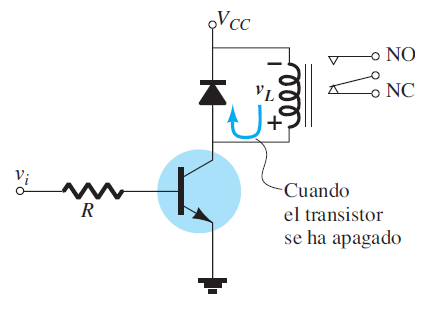
\includegraphics[width=0.5\textwidth]{figuras/aplicaciones_2.png}
\end{figure}

\end{frame}


\begin{frame}{Foco halógeno con termistor de protección}

\begin{figure}[H]
    \centering
    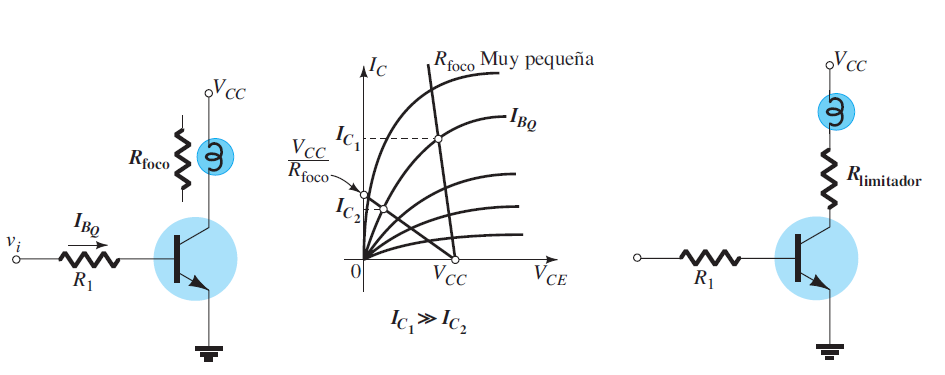
\includegraphics[width=\textwidth]{figuras/aplicaciones_3_foco_termistor.png}
\end{figure}

\end{frame}


\begin{frame}{Fuente de corriente constante}

\begin{figure}[H]
    \centering
    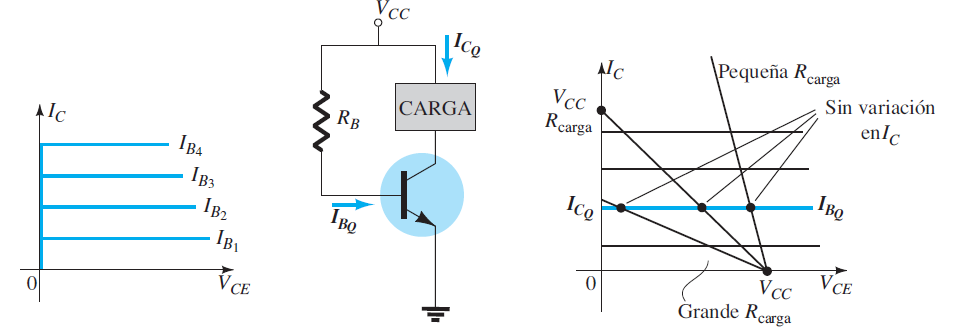
\includegraphics[width=\textwidth]{figuras/aplicaciones_4_fuente_i_constante.png}
\end{figure}

\end{frame}


\begin{frame}{Fuente de corriente constante por divisor de tensión}

\begin{figure}[H]
    \centering
    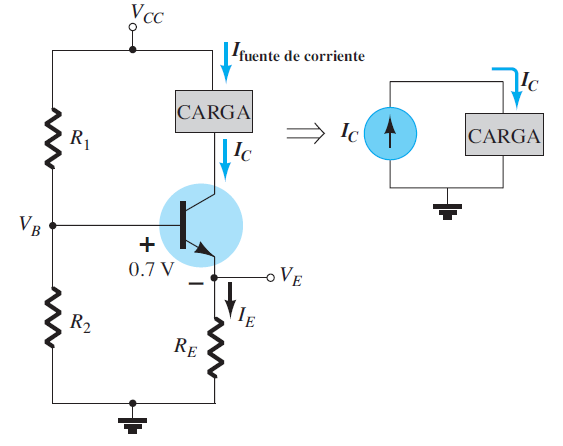
\includegraphics[width=0.6\textwidth]{figuras/aplicaciones_5_fuente_i_constante.png}
\end{figure}

\end{frame}


\begin{frame}{Alarma con comparador de corriente de referencia}

\begin{figure}[H]
    \centering
    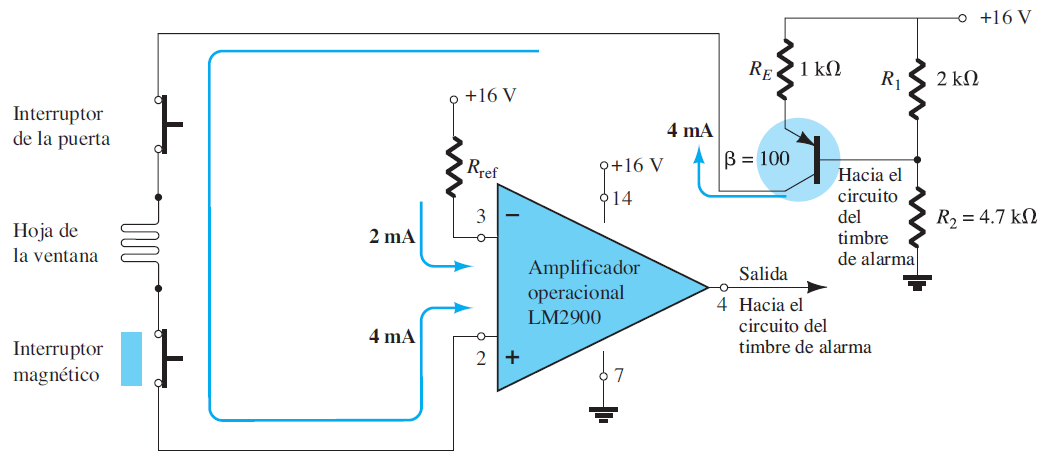
\includegraphics[width=\textwidth]{figuras/aplicaciones_6_alarma_comparador.png}
\end{figure}

\end{frame}


\begin{frame}{Compuertas lógicas}

\begin{columns}

\begin{column}{0.5\textwidth}

\begin{figure}[H]
    \centering
    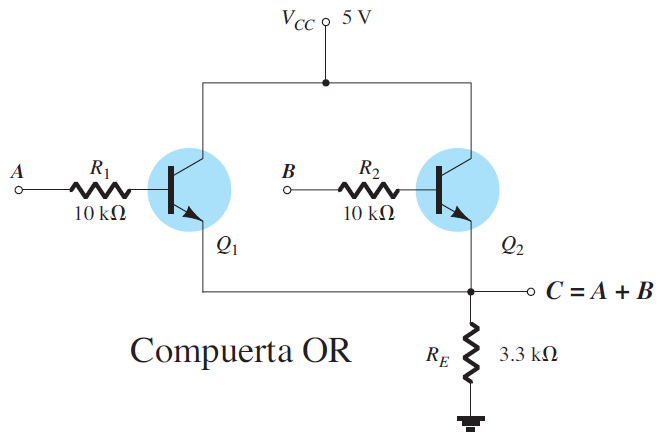
\includegraphics[width=\textwidth]{figuras/aplicaciones_7_compuertas.png}
\end{figure}

\end{column}

\begin{column}{0.5\textwidth}

\begin{figure}[H]
    \centering
    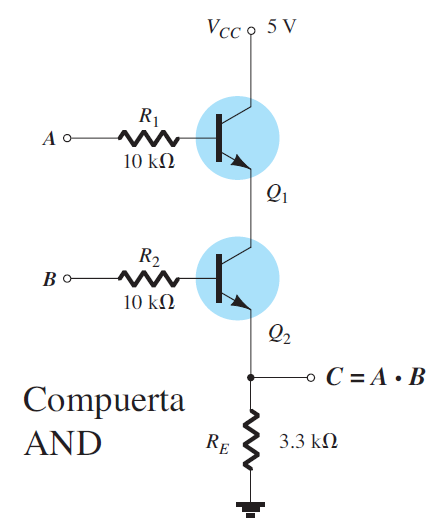
\includegraphics[width=0.7\textwidth]{figuras/aplicaciones_8_compuertas.png}
\end{figure}

\end{column}

\end{columns}

\end{frame}


\begin{frame}{Espejo de corriente}

\begin{figure}[H]
    \centering
    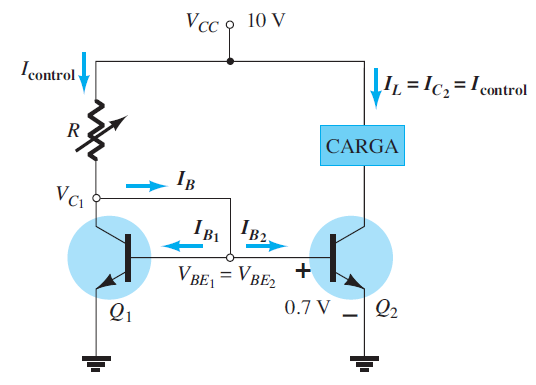
\includegraphics[width=0.5\textwidth]{figuras/aplicaciones_9_espejo.png}
\end{figure}

\end{frame}


\begin{frame}{Indicador de nivel}

\begin{figure}[H]
    \centering
    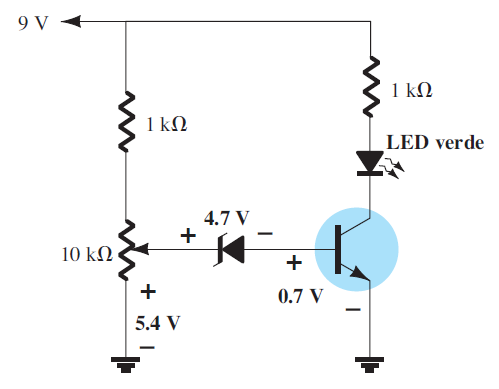
\includegraphics[width=0.5\textwidth]{figuras/aplicaciones_10_indicador_nivel.png}
\end{figure}

\end{frame}


\begin{frame}{Lecturas recomendadas}

\begin{itemize}
    \item Boylestad, R. and Nahelsky, L. Electrónica: teoría de circuitos y dispositivos electrónicos, 10ma ed., Capítulo 4: Polarización de cd de los transistores BJT, pp. 220-227, Pearson Educación, México, 2009.
\end{itemize}

\end{frame}

\end{document}
